\documentclass[a4paper,11pt,twocolumn]{article}
\usepackage{polyglossia} % Eesti keele tugi
\setdefaultlanguage{estonian}
\usepackage{geometry}% Paigutus
\usepackage{graphicx}% Joonised
\graphicspath{ {images/} }
\usepackage{csquotes}% Eesti jutumärgid \enquote{}
\usepackage{enumitem}% Listid
\usepackage[compact]{titlesec}% Kompaktsed pealkirjad
\usepackage{siunitx}% SI ühikud
\usepackage{tikz}
\usepackage[siunitx]{circuitikz}
\usepackage[final]{microtype}
\usepackage{amsmath}
\usepackage{lmodern}
\geometry{
    paper=a4paper, % Paper size, change to letterpaper for US letter size
    top=0.5cm, % Top margin
    bottom=1cm, % Bottom margin
    left=0.5cm, % Left margin
    right=0.5cm, % Right margin
    foot=0.5cm, % Footer-margin distance
    %showframe, % Uncomment to show how the type block is set on the page
}


%\setlength{\intextsep}{0pt}

\setlength{\parindent}{0cm}% Taandridu pole
\setlength{\parskip}{1em}% Paragraafide vahed
\setlist[itemize]{topsep=0em, partopsep=0em, parsep=0em, itemsep=0.5em}% Itemize spacing

\usepackage{xparse}

% Ülesanded \begin{question}[viide][joonis][joonise suurus] (võib olla ka ainult [viide] või [joonis][joonise suurus])
\newcounter{myproblems}
\NewDocumentEnvironment{question}{o o o}
{\par \refstepcounter{myproblems} \textbf{Ülesanne \themyproblems .} \ignorespaces\IfValueT{#1}{\IfValueTF{#3}{\textbf{(#1)} \ignorespaces}{\IfNoValueT{#2}{\textbf{(#1)} \ignorespaces}}}}
{\IfValueT{#2}{\IfValueTF{#3}{\begin{figure}[h!]\includegraphics[width=#3]{#2.pdf}\centering\vspace{-1em}\end{figure}}{\begin{figure}[h!]\includegraphics[width=#2]{#1.pdf}\centering\vspace{-1em}\end{figure}}}\ignorespacesafterend}

% Alaülesanded
\newenvironment{subquestion}
{\setlength{\parskip}{0pt}\begin{enumerate}[label=\alph*), nolistsep]}
{\end{enumerate}\setlength{\parskip}{1em}\ignorespacesafterend}

% Vihjete jaoks
\newenvironment{hint}[1][Vihje]
{\setlength{\parskip}{0em} \textit{#1}: \ignorespaces}
{\setlength{\parskip}{1em}\ignorespacesafterend}

\newcommand{\pvec}[1]{\vec{#1}\mkern2mu\vphantom{#1}}% Primed vector

% Lahendused jaoks
\usepackage{hyperref}
\newenvironment{solutions}
{\begin{enumerate}[label=\textbf{\arabic*.}, wide]}
{\end{enumerate}}

% Displaystyle valemite paigutus
\makeatletter
\g@addto@macro{\normalsize}{%
    \setlength{\abovedisplayskip}{4pt}
    \setlength{\abovedisplayshortskip}{4pt}
    \setlength{\belowdisplayskip}{4pt}
    \setlength{\belowdisplayshortskip}{4pt}
    }
\makeatother

% \directlua{dofile("DetectUnderfull.lua")}
\tikzset{
    odot/.style={
        circle,
        inner sep=0pt,
        node contents={$\odot$},
        scale=1
    },
    otimes/.style={
        circle,
        inner sep=0pt,
        node contents={$\otimes$},
        scale=1
    }}

\usepackage{blindtext}

\begin{document}
{\huge \textbf{Calculus}\hfill \normalsize {nr 1}} \\
{Jarl Patrick Paide \hfill 14. jaanuar 2020}

\section{Tuletis}

Tuletis näitab funktsiooni muutumise kiirust. Graakifult vaadates on tuletis mingi funktsiooni puutuja tõus mingis punktis. Tuletist võttes saame me uus funktsiooni mis näitab seda tõusu sõltuvuses $x$'ist. Kui meil on funktsioon $f(x)$ siis on selle funktsiooni tuletis $f'(x)$ on deffineeritud järgnevalt
\begin{equation*}
f'(x) = \lim_{\Delta x \to 0} \frac{\Delta y}{\Delta x} = \lim_{\Delta x \to 0} \frac{f(x+\Delta x) - f(x)}{\Delta x}
\end{equation*}
$\Delta x$ asemel võib kasutada tähist $dx$, kui muutus on väga väike
\begin{equation*}
\lim_{\Delta x \to 0} \Delta x = dx
\end{equation*}

Seega kui me võtame tuletis funktsioonist $f(x)$, $x$'i järgi siis saab seda tähistada järgnevalt
\begin{equation*}
f'(x)=\frac{d}{dx}f(x) = \frac{f(x+ dx) - f(x)}{dx}
\end{equation*}

Vaatame, kuidas me saame kasutades tuletis deffinitsiooni leida lihtsa tuletise funktsioonist $f(x) = x$

\begin{equation*}
f'(x) = \frac{(x+dx) - (x)}{dx} = \frac{dx}{dx} = 1
\end{equation*}

Kui mõelda selle funktsiooni graafikule siis on see vastus usutav ja loogiline.

\subsection{Konstandid}
Kui meil on funktsioon $f(x) = a$ siis on see funktsioon konstantne. Graafikul vaadates on tegemist x-teljega paralleelse sirgega, mis läbib y-telge punktis a. Kuna selle funktsiooni tõus igas punnktis on 0, siis on selle funktsiooni tuletis $f'(x) = 0$

Kui meil on funktsioon $f(x) = ag(x)$ siis kasutades tuletise deffinitsiooni saame teha järgnevat
\begin{equation*}
f'(x) = \frac{ag(x+dx)-ag(x)}{dx} = a\frac{g(x+dx)-g(x)}{dx}=ag'(x)
\end{equation*}
Ehk siis kui meil funktsioon $f(x) = ag(x)$ siis me saame tuua konstanti ette ja võtta tuletist ülejäänud funktsioonist.

\subsection{Polünomid}
Vaatame lihtsat funktsiooni $f(x) = x^2$ ja võttame sellest funktsioonist tuletist tuletise deffinitsiooni abiga
\begin{multline*}
f'(x) = \frac{(x+dx)^2-(x)^2}{dx} = \frac{x^2 + 2xdx + dx^2 - x^2}{dx} = \\
= 2x + dx = 2x
\end{multline*}

Kui $x=0$ siis see funktsioon fuutub x-telge, seega on loogiline, et tuletis, ehk tõus, on selles punktsi 0. Kui $x=1$ siis on funktsiooni väärtus 1, aga tõus selles punktis on 2. See funktsioon kahaneb vahemikus $x<0$ seega on loogiline, et seal on funktsiooni tuletis negatiivne. Vastupidi jällegi juhul kui $x>0$. Ning mida suuremaks x muutub seda kiiremini hakkab funktsioon muutuma, seega funktsiooni puutuja tõus suureneb.

Vaatame nüüd polünomi üldjuhtu $f(x) = x^n$
\begin{multline*}
f'(x) = \frac{(x+dx)^n-x^n}{dx} = \frac{(x^n+nx^{n-1}dx+...+dx^n)-x^n}{dx}= \\
=nx^{n-1}+(n(n-1)/2)x^{n-2}dx+...+dx^{n-1}= nx^{n-1}
\end{multline*}
Seega $\frac{d}{dx}(x^n)=nx^{n-1}$, ehk kui $f(x)=2x^3$ siis $f'(x)=6x^2$.

\subsection{Funktsioonide liitmine}
Olgu meil funktsioon $f(x) = g(x) + h(x)$ ja vaatame, kuidas leida tuletist $f'(x)$
\begin{multline*}
f'(x) = \frac{(g(x+dx)+h(x+dx))-(g(x)+h(x))}{dx} = \\
= \frac{g(x+dx) - g(x)}{dx} + \frac{h(x+dx) - h(x)}{dx} = g'(x) + h'(x)
\end{multline*}
Seega kui funktsioon on funktsioonide summa siis on selle funktsiooni tuletis nende summa liikmete tulemiste summa.

\subsection{Funkstioonide korrutamine}
Olgu meil funktsioon $f(x) = g(x)h(x)$ ja vaatame, kuidas leida tuletist $f'(x)$
\begin{equation*}
f'(x) = \frac{(g(x+dx)h(x+dx)) - (g(x)h(x))}{dx} = 
\end{equation*}
Me võime liita ja lahutada murru lugejast sama arvu $g(x)h(x+dx)$ ja me teame, et suvaline funktsioon $k(x+dx) = k(x)$ seega saame
\begin{multline*}
= \frac{g(x+dx)h(x+dx) - g(x)h(x+dx) + g(x)h(x+dx) - g(x)h(x)}{dx} = \\
= \frac{h(x+dx)(g(x+dx)-g(x))}{dx} + \frac{g(x)(h(x+dx)-h(x))}{dx} = \\
= g'(x)h(x) + g(x)h'(x)
\end{multline*}
Seeda saab lihtsamalt kirjutada. Kui meil on funktsioonid $u$ ja $v$, mis mõlemad sõltuvad $x$'ist, siis $(uv)' = u'v + uv'$.

\subsection{Liitfunktsioonid ?}
Olgu meil funktsioon $f(x) = g(h(x))$. Näiteks, seega kui $h(x) = x+1$ ja $g(x) = x^2$ siis $f(x) = g(x+1) = (x+1)^2$. Nüüd vaatame, kuidas sellisest funktsioonist tuletist võtta. Tuletise deffinitsioonist saame
\begin{equation*}
f'(x) = \frac{g(h(x+dx)) - g(h(x))}{h(x+dx) - h(x)} \cdot \frac{h(x+dx) - h(x)}{dx}
\end{equation*}
Kui me teeme asenduse $h(x) = a$ ja $h(x+dx) = a + da$, siis saame, et
\begin{multline*}
f'(x) = \frac{g(a+da) - g(a)}{da} \cdot \frac{h(x+dx) - h(x)}{dx} = \\
= \frac{dg(a)}{da}\cdot\frac{da}{dx} = \frac{dg(h(x))}{dh(x)}\cdot\frac{dh(x)}{dx}
\end{multline*}
Kuna sellest võib olla raske aru saada teeme läbi ühe näite. Olgu meil funktsioon $f(x) = (x+1)^2$, ja võtame $h(x) = x+1$ ja $g(x) = x^2$ siis $f(x) = g(h(x))$. Me võime teha asenduse $a = h(x)$. Seega tuletis on 
\begin{multline*}
f'(x) = \frac{d(x+1)^2}{d(x+1)} \cdot \frac{d(x+1)}{dx} = \frac{d a^2}{da} \cdot \frac{d(x+1)}{dx} =\\
= (2a) \cdot (1+0) = 2(x+1) = 2x+2
\end{multline*}
Kuna me oskame nüüd ka teist moodi seda tuletist võtta teeme kontrolliks ka selle läbi
\begin{equation*}
((x+1)^2)' = (x^2 + 2x + 1)' = (x^2)' + (2x)' + (1)' = 2x + 2
\end{equation*}
Seega kõik töötab

\subsection{Funktsioonide jagamine}
Vaatame nüüd jagatist $\frac{u}{v}$ ja leiame selle tuletise.
\begin{equation*}
(\frac{u}{v})'= (u\cdot\frac{1}{v})'=u'(\frac{1}{v})+u(\frac{1}{v})'
\end{equation*}
Kuna $\frac{1}{v}$ on liitfunktsoon siis selle tuletis on
\begin{equation*}
(\frac{1}{v})' = \frac{d (1/v)}{dv} \cdot \frac{dv}{dx} = \frac{-1}{v^2} \cdot v'
\end{equation*}
Seega on jagatise tuletis 
\begin{equation*}
(\frac{u}{v})'=u'(\frac{1}{v})+u(\frac{1}{v})' = \frac{u'v-uv'}{v^2}
\end{equation*}

\subsection{Sin ja Cos}
Siinuse ja Cosiinuse summa abivalemid
\begin{equation*}
\sin(\alpha\pm\beta) = \sin(\alpha)\cos(\beta)\pm\sin(\beta)\cos(\alpha)
\end{equation*}
\begin{equation*}
\cos(\alpha\pm\beta) = \cos(\alpha)\cos(\beta)\mp\sin(\alpha)\sin(\beta)
\end{equation*}
Võtame funktsioonist $f(x) = \sin(x)$ tuletist kasutades tuletise deffinitsiooni
\begin{equation*}
f'(x) = \frac{\sin(x+dx)-\sin(x)}{dx} =
\end{equation*}
Kuna $dx$ läheneb nullile siis $\cos(dx) = 1$ ja $\sin(dx)/dx=1$ ja sellest saame, et 
\begin{equation*}
= \frac{\sin(x)\cos(dx)+\cos(x)\sin(dx)-\sin(x)}{dx} = \cos(x)
\end{equation*}

Vaatame nüüd juhtu $f(x) = \cos(x)$
\begin{multline*}
f'(x) = \frac{\cos(x+dx)-\cos(x)}{dx} = \\
= \frac{\cos(x)\cos(dx) - \sin(x)\sin(dx) - \cos(x)}{dx} = -\sin(x)
\end{multline*}
Kuna me saame konstantid tuletiest välja võtta saame, et $(-\sin(x))' = -\cos(x)$ ja $(-\cos(x))' = \sin(x)$. Kuna ülejäänud trigonomeetrilisi võrrandeid saab nende kahe abil leida, siis piisab nende kahe tuletisest. Leiame näiteks $\tan(x)$ tuletise
\begin{multline*}
\tan(x)'=(\frac{\sin(x)}{\cos(x)})'  = \frac{\sin(x)'\cos(x)-\cos(x)'\sin(x)}{\cos^2(x)}=\\
=\frac{\cos^2(x) + \sin^2(x)}{\cos^2(x)} = \sec^2(x)
\end{multline*}

\subsection{Logarütm}
Nüüd vaatame logarütmilisi funktsioone. Alustame funktsioonist $f(x) = \ln x$. Selle jaoks meil vaja $e$ deffinitsiooni, mis on järgnev
\begin{equation*}
e=\lim_{n \to \infty}(1+\frac{1}{n})^n \approx 2.718281828459...
\end{equation*}
Kasutades tuletise deffinitsiooni saame järgneva
\begin{multline*}
  f'(x)=\frac{\ln(x+dx) - \ln(x)}{dx}=\frac{1}{dx}\ln(1-\frac{dx}{x})=\\
  =\ln((1+\frac{dx}{x})^{\frac{1}{dx}}
\end{multline*}
Teeme nüüd asenduse $u=\frac{x}{dx}$
\begin{equation*}
\ln((1+\frac{dx}{x})^{\frac{1}{dx}})=\lim_{u \to \infty}\ln((1+\frac{1}{u})^{\frac{u}{x}}) = \lim_{u \to \infty}\frac{1}{x}\ln((1+\frac{1}{u})^{u})=
\end{equation*}
Märkame, et viimase logarütmi sees on $e$, seega jätkame
\begin{equation*}
=\frac{\ln(e)}{x}=\frac{1}{x}
\end{equation*}
Nüüd leiame tuletise suvalisele logarütmile $f(x)=\log_{a}(x)$
\begin{equation*}
f'(x)=(\log_{a}(x))'=(\frac{\ln(x)}{\ln(a)})'=
\end{equation*}
Kuna aga $\ln(a)$ on konstant, võib selle välja tuua ja siis saame
\begin{equation*}
=\frac{1}{\ln(a)}(\ln(x))'=\frac{1}{\ln(a)x}
\end{equation*}

\subsection{eksponendid}
Nüüd vaatame eksponentfunktsioone. Alustame funktsiooniga $f(x)=e^x$. Liitfunktsiooni tuletisest me teame järgnevat
\begin{multline*}
  (\ln(e^x))'=\frac{1}{e^x}(e^x)'\\
  (x)'e^x=(e^x)'\\
  (e^x)'=e^x
\end{multline*}
Vaatame nüüd funktsiooni $f(x)=a^x$. Me saame seda funktsiooni ümber kirjutada kujul $f(x)=e^{x\ln(a)}$.
\begin{multline*}
f'(x)=(e^{x\ln(a)} )'=e^{x\ln(a)}(x\ln(a))'=a^x\ln(a)
\end{multline*}

\subsection{Kokkuvõte}
Nüüd me oleme tõestanud ja näidanud, kuidas võtta elementaarfunktsioonidest tuletise ja kuidas võtta mitmset erinevast funktioonist koosnevast fuktsioonist tuletist. Seega nüüd on oskus võtta kõigist funktsioonidest tuletist. Et võtta kõik kokku on järgnev kokkuvõttev tabel. ($u$ ja $v$ on tabelis x sõltuvad erinevad funktsioonid)

\begin{table}[h]
  \centering
  \caption{Põhifunktsioonide tuletised}
  \begin{tabular}{c | c}
    \hline
    funktsioon & tuletis\\
    \hline
    $(cu)'$ & $cu'$\\
    $(u+v)'$ & $u'+v'$\\
    $(uv)'$ & $u'v+v'u$\\
    $(u/v)'$ & $(u'v-v'u)/v^2$\\
    $du(v)/dx$ & $(du/dv)(dv/dx)$\\
    \hline
    $c$ & $0$\\
    $x^n$ & $nx^{n-1}$ \\
    $\sin x$ & $\cos x$\\
    $\cos x$ & $-\sin x$\\
    $\tan x$ & $\sec^2 x$\\
    $\ln x$ & $1/x$\\
    $\log_a x$ & $1/(x\ln a)$\\
    $e^x$ & $e^x$\\
    $a^x$ & $e^x\ln a$    
  \end{tabular}
\end{table}

\section{Tuletise rakendused ja ülesanded}
Nüüd, kus meil on matemaatilised võtted selged vaatame, kuidas tuletisi rakendada.

\subsection{Funktsiooni maksimumid ja miinimumid}
Funktsiooni lokaalne miinimum ja maksimum on kohtades, kus funktsiooni graafik on horisontaalne, ehk nendes punktides on tuletis $0$. Punkte, kus funktsiooni tuletis on $0$ nimetatakse ekstreemumisteks. Kuid funktsiooni maksimaalne väärtus ei pruugi olla  ekstreemum kohas.

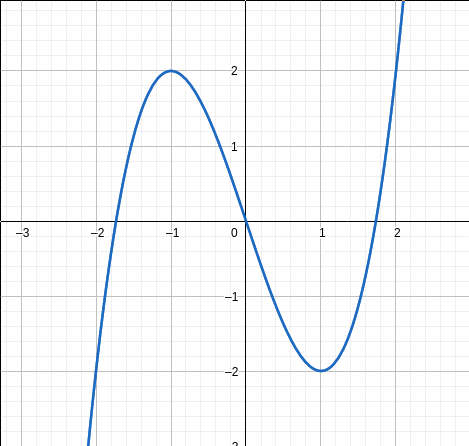
\includegraphics[width = .4\textwidth]{joon1.png}

Vaatame lähemalt funktsiooni $f(x)=x^3-3x$. Sellel funktsioonil on kahes kohas lokaalne miinimum. Selle funktsiooni tuletis on $f'(x)=3x^2-3$. Seades selle nulliks saame kaks lahendi $x_1=1$ ja $x_2=-1$. Nendes kahes punktis on selle funktsiooni lokaalne miinimum, aga mitte globaalne miinimum. Et teha kindlaks, mis on selle funktsiooni minimaalne ja maksimaalne väärtus tuleb vaadata ka juhte $x=-\infty$ ja $x=\infty$. Paneme saadud $x$'i väärtused tabelisse ja leiame $f(x)$ väärtuse.
\begin{table}[h]
  \centering
  \begin{tabular}{c | c c c c}
    $f(x)$ & $-\infty$ & $-1$ & $1$ & $\infty$\\
    \hline
    $x$ & $-\infty$ & $2$ & $-2$ & $\infty$    
  \end{tabular}
\end{table}
Näeme tabelis ja joonisest, et $-1$ ja $1$ on küll vastavalt lokaalne miinimum ja maksimum, kuid seal ei ole funktsiooni minimaalne ega maksimaalse väärtus.

\begin{question}
  Leia parabooli $f(x)=ax^2+bx+c$ haripunkti $x$ kordinaat
\end{question}
\textbf{Lahendus:} Võtame funktsioonist $f(x)$ tuletist ja pananeme võrduma $0$'ga. Saame $2ax+b=0$ ja siit avaldame $x=\frac{-b}{2a}$. Saadud lahend näitab parabooli lokaalset miinimumi või maksimumi (vastavalt a märgile) ning see ekstreemum on ka samas haripunkt. Vastus on seega $x=\frac{-b}{2a}$.

\subsection{funktsiooni kumerus}
Funktsioon on mingis punktsi kas kumer, nõgus või sirge. Funktsiooni kumerus näitab, funktsiooni tõusu muutumise kiirust. Kui $x$ suureneb, siis kumera funktsiooni tõus suureneb, nõguse funktsiooni tõus vähemeb ja sirgel tõus ei muutu.  Näide kumerast funktsioonist on $f(x)=x^2$ ja näide nõgusast funktsioonist on $f(x)=-x^2$.

Nüüd vaatame, kuidas leida, kas funktsioon on nõgus või kõver. Kui meil on funktsioon $f(x)$ siis selle funktsiooni tuletis on $f'(x)$. Kuna me tahame teada, kas see tõus on suurenev või vähenev siis me võtame sellest funktsioonist teise tuletise $f''(x)$. Kui $f''(x) > 0$ siis on algse funktsiooni tõus suurenemas (funktsioon on kumer) ja kui $f''(x) < 0$ siis on see vähenemas (funktsioon on nõgus).

Vaatame näiteks tuttavat funktsiooni $f(x) = x^3 - 3x$. Jooniselt näeme juba, et mingis piirkonnas on see fuktsioon kumer ja mingis piirkonnas on see funktsioon nõgus. Võtame esimese tuletise $f'(x) = 3x^2 - 3$ ja teise tuletise $f''(x) = 6x$. Näeme, et piirkonnas $x < 0$ on $f''(x) < 6$ ehk funktsioon on nõgus, piirkonnas $x=0$ on $f(x) = 0$ ehk funktsioon on sirge ja piirkonnas $x>0$ on $f(x) > 0$ ehk funktsioon on kumer.

Funktsiooni kumerus näitab meile, kas ekstreemumpunkt on lokaalne miinimum või maksimum (või kumbki näiteks $f(x) = x^3$ punkt $x=0$). Kui ekstreemumpunkt asub kumera funktsiooni peal on tegu lokaalse miinimumiga ja kui ekstreemum on nõguse funktsiooni peal on tegu lokaalse maksimumiga. Kontrolliks võib vaadelda eelnevalt mainitud funktsiooni.

\subsection{Näiteid füüsikast}
Tuletis näitab kui palju muutub funktisooni väärtus väikese sisendi muuuse korral. Kiirus näitab kuidas muutub asukoht väikese aja muudu korral. Kiirus on asukoha muut aja suhtes, ehk asukoha tuletis aja järgi. Me teame, et me saame asukohta mingil ajahetkel leiga valemiga

\begin{equation}
x(t) = x_0 + vt + \frac{at^2}{2}
\end{equation}

Kui me võtame sellest funktioonist tuletise, siis saame kiiruseks mingil ajahetkel $v(t) = x'(t) = v + at$. Ning samas kiiruse muutus aja jooksul, ehk  kiiruse tuletis aja järgi on kiirendus. Selleks saame $a(t) = v'(t) = x''(t) = a$.

Me saame vedru küljes oleva punkti asukohta kirjeldada ajas $x(t)=A\sin(\omega t)$. Seega me saame leida punkti kiiruse võttes funktioonist tuletist $v(t)=x'(t)=A\omega\cos(\omega t)$ ja saame leida ka kiirenduse $a(t)=v'(t)=-A\omega^2\sin(\omega t)$. Mõeldes loogiliselt on valemid tõesed, sest kui $|\sin(x)|$ on maksimaalne siis $\cos(x) = 0$ ja vastupidi, seega kui kiirus on null (vedru on maksimaalselt välja venitatud või kokku lükkatud) on asukoha ja kiirenuse absoluutväärtus maksimaalne.

\subsection{Ülesanded}
\begin{question}
Olgu meil anum, mis on tagurpidi keeratud koonus, mille põhja raadius on $R = 4 m$ ja kõrgus on $H = 10 m$. Seda anumat täidetakse kraanist, kust väljub $v = 0.1 m^3/s$ vett. Leia kui kiiresti tõuseb veepiiri kiirus.
\end{question}

\textbf{Lahendus:} Koonuse ruumala valem on $V=\pi r^2h/3$. Me teame, et koonuse raadius sõltub kõrgusest $r(h)=hR/H$. Seega me saame, et kui veega on täidetud kõrguseni $h$ siis on vee ruumala $V(h)=\frac{\pi R^2}{3H^2}h^3$. Võttes tuletist saame $\frac{dV}{dt} = \frac{\pi R^2h^2}{H} \frac{dh}{dt}$ ja me teame, et $v= \frac{dV}{dt}$, seega me saame avaldada kõrguse kiiruse muutu ja see on $\frac{dh}{dt} = \frac{v H^2}{\pi r^2 h^2} = \frac{5}{\pi 8 h^2} (\frac{m}{s})$.


\end{document}
